%%%%%%%%%%%%%%%%%%%%%%%%%%%%%%%%%%%%%%%%%
% Beamer Presentation
% LaTeX Template
% Version 1.0 (10/11/12)
%
% This template has been downloaded from:
% http://www.LaTeXTemplates.com
%
% License:
% CC BY-NC-SA 3.0 (http://creativecommons.org/licenses/by-nc-sa/3.0/)
%
%%%%%%%%%%%%%%%%%%%%%%%%%%%%%%%%%%%%%%%%%

%----------------------------------------------------------------------------------------
%	PACKAGES AND THEMES
%----------------------------------------------------------------------------------------

\documentclass{beamer}

\mode<presentation> {

% The Beamer class comes with a number of default slide themes
% which change the colors and layouts of slides. Below this is a list
% of all the themes, uncomment each in turn to see what they look like.

%\usetheme{default}
%\usetheme{AnnArbor}
%\usetheme{Antibes}
%\usetheme{Bergen}
%\usetheme{Berkeley}
%\usetheme{Berlin}
%\usetheme{Boadilla}
%\usetheme{CambridgeUS}
%\usetheme{Copenhagen}
%\usetheme{Darmstadt}
%\usetheme{Dresden}
%\usetheme{Frankfurt}
%\usetheme{Goettingen}
%\usetheme{Hannover}
%\usetheme{Ilmenau}
%\usetheme{JuanLesPins}
%\usetheme{Luebeck}
\usetheme{Madrid}
%\usetheme{Malmoe}
%\usetheme{Marburg}
%\usetheme{Montpellier}
%\usetheme{PaloAlto}
%\usetheme{Pittsburgh}
%\usetheme{Rochester}
%\usetheme{Singapore}
%\usetheme{Szeged}
%\usetheme{Warsaw}

% As well as themes, the Beamer class has a number of color themes
% for any slide theme. Uncomment each of these in turn to see how it
% changes the colors of your current slide theme.

%\usecolortheme{albatross}
%\usecolortheme{beaver}
%\usecolortheme{beetle}
%\usecolortheme{crane}
%\usecolortheme{dolphin}
%\usecolortheme{dove}
%\usecolortheme{fly}
%\usecolortheme{lily}
%\usecolortheme{orchid}
%\usecolortheme{rose}
%\usecolortheme{seagull}
%\usecolortheme{seahorse}
%\usecolortheme{whale}
%\usecolortheme{wolverine}

%\setbeamertemplate{footline} % To remove the footer line in all slides uncomment this line
%\setbeamertemplate{footline}[page number] % To replace the footer line in all slides with a simple slide count uncomment this line

%\setbeamertemplate{navigation symbols}{} % To remove the navigation symbols from the bottom of all slides uncomment this line
}

\usepackage{graphicx} % Allows including images
\usepackage{booktabs} % Allows the use of \toprule, \midrule and \bottomrule in tables
\usepackage[utf8]{inputenc}
\usepackage[T1]{fontenc}
\usepackage[]{algorithm2e}
\usepackage{multicol}

%----------------------------------------------------------------------------------------
%	TITLE PAGE
%----------------------------------------------------------------------------------------

\title[PIDR]{Développement d’un outil d’édition et de manipulation de réseaux bayésiens} % The short title appears at the bottom of every slide, the full title is only on the title page

\author{R. AGATHON V. WEGMANN-SERIN} % Your name
{

}

\begin{document}

\begin{frame}
\titlepage % Print the title page as the first slide
\end{frame}

\begin{frame}
\frametitle{Plan} % Table of contents slide, comment this block out to remove it
\tableofcontents % Throughout your presentation, if you choose to use \section{} and \subsection{} commands, these will automatically be printed on this slide as an overview of your presentation
\end{frame}

%----------------------------------------------------------------------------------------
%	PRESENTATION SLIDES
%----------------------------------------------------------------------------------------

%------------------------------------------------
\section{Contexte/Problématique}

\begin{frame}
\frametitle{Contexte/Problématique}
\begin{block}{Sujet du PIDR}
Description : Au sein du laboratoire (CRAN), nous utilisons régulièrement des outils basés sur des
graphes probabilistes ou quasi-probabilistes. Nous avons besoin d’un outil qui permet de créer les
graphes et les données probabilistes ou quasi-probabiliste sous java/matlab pour réaliser des modèles
utiles à la communauté internationale travaillant sur le sujet. L’objectif est de créer un outil logiciel opensource
mis à la disposition de la communauté scientifique.
\end{block}

\end{frame}

%------------------------------------------------

\section{Définitions}

\begin{frame}
\frametitle{Réseaux bayésiens}
\end{frame}

\begin{frame}
\frametitle{Inférence}
\end{frame}

%------------------------------------------------

\section{Analyse des outils existants}

\begin{frame}
\frametitle{Analyse des outils existants}

\textbf{Spécificités des boites à outils d'édition de réseau bayésien}
\begin{itemize}
\item Langage de programmation 
\item Interface graphique 
\item Prix
\item Open source 
\end{itemize}

\end{frame}

\begin{frame}
\frametitle{Java Bayes}

\begin{figure}
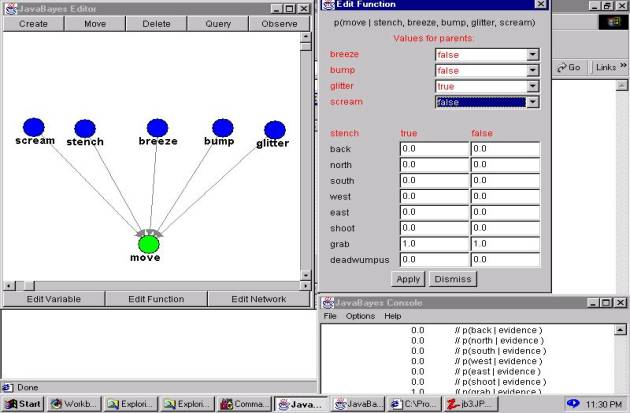
\includegraphics[width=0.9\linewidth]{javabayes.jpg}
\end{figure}

\end{frame}

%------------------------------------------------

\begin{frame}
\frametitle{BayesiaLab}

\begin{figure}
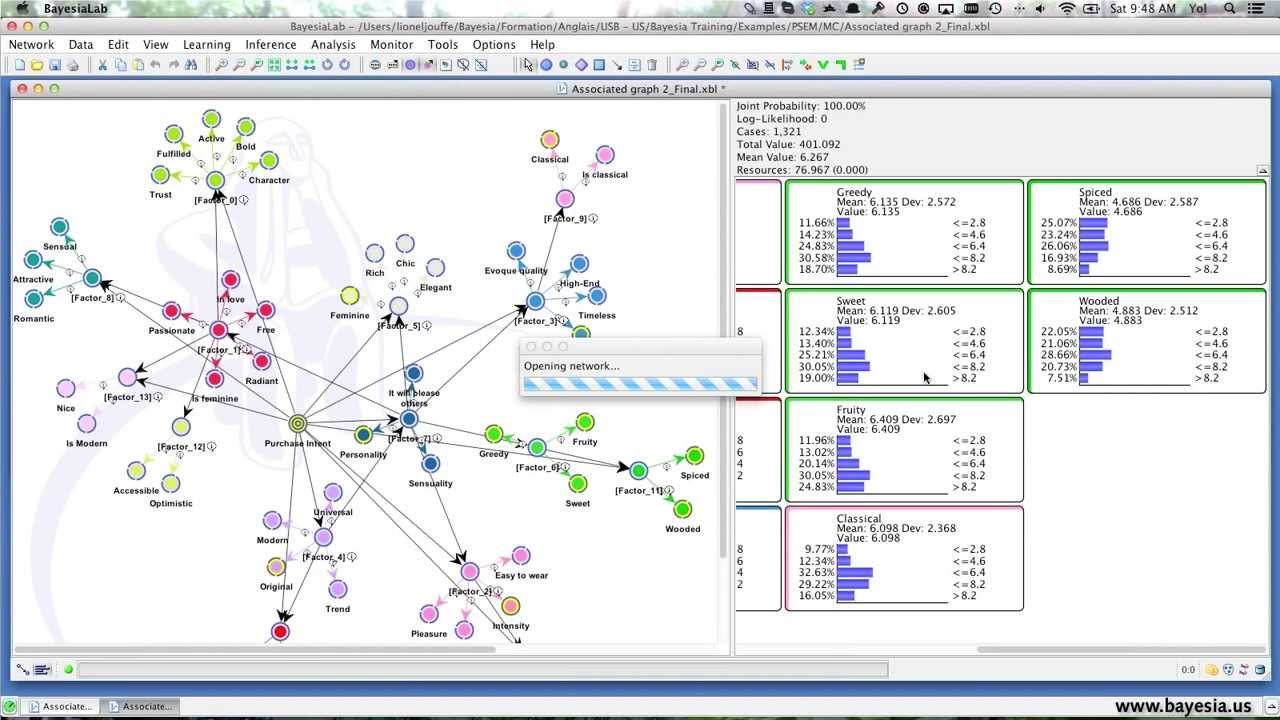
\includegraphics[width=1.0\linewidth]{bayesialab.jpg}
\end{figure}

\end{frame}

%------------------------------------------------

\section{Présentation de l'outil DynGraph}

\begin{frame}
\frametitle{Présentation de l'outil DynGraph}
\begin{columns}[c] % The "c" option specifies centered vertical alignment while the "t" option is used for top vertical alignment

\column{.40\textwidth} % Left column and width
\textbf{Heading}
\begin{enumerate}
\item Statement
\item Explanation
\item Example
\end{enumerate}

\column{.6\textwidth} % Right column and width
\begin{figure}
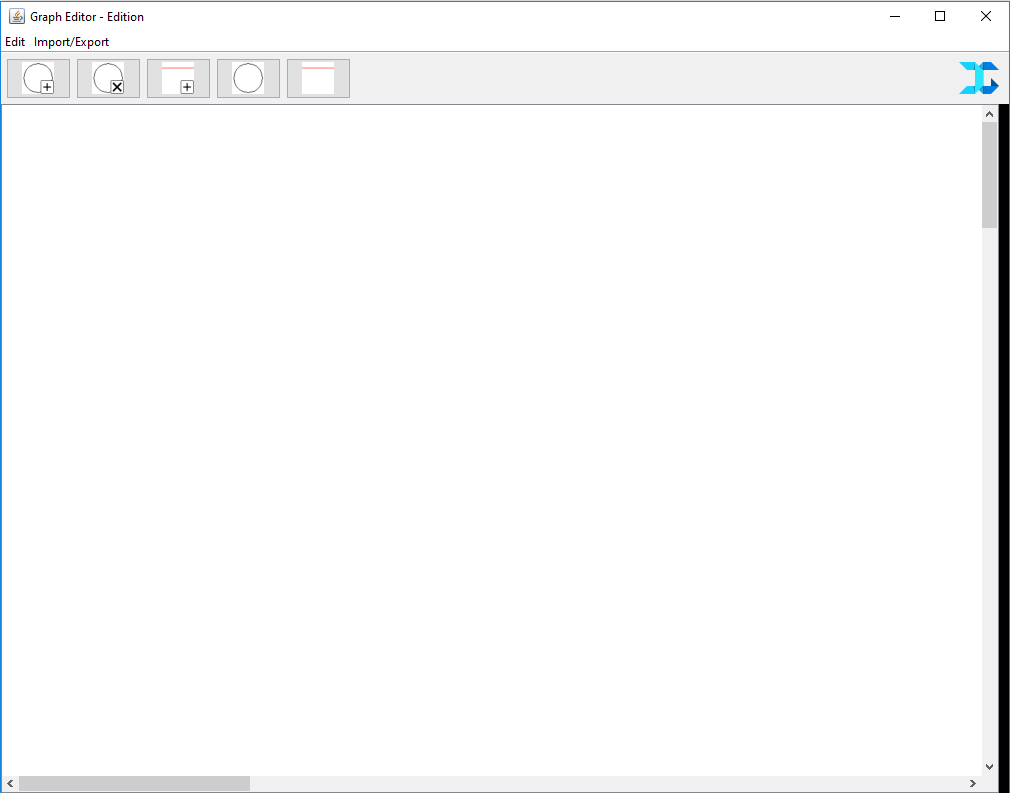
\includegraphics[width=1.0\linewidth]{Dyngraph.png}
\end{figure}
\end{columns}
\end{frame}

%------------------------------------------------

\section{Méthodologie}

	\subsection{Implémentation des réseaux bayésiens et des calculs d'inférence }
	
	\begin{frame}
	\frametitle{Implémentation des réseaux bayésiens et des calculs d'inférence }
	
	\textbf{Processus}
	
	\begin{enumerate}
	\item Détection de cycle dans le graphe 
	\item Transformation du graphe en réseau bayésien
	\item Édition des tables de probabilités 
	\item Calcul d'inférence 
	\end{enumerate}		
	
	\end{frame}
	
%------------------------------------------------	
	
	
	\begin{frame}
	\frametitle{Algorithme de détection de cycle}
		
		\begin{block}{algorithme de détection de cycle Entrée/Sortie}
		
		\begin{algorithm}[H]
 \KwData{Graphe G contenant une liste de nœuds et une liste d'arcs}
 \KwResult{liste des nœuds à problème : N}
\end{algorithm}
		
		\end{block}
	
	\end{frame}

		\begin{frame}
	\frametitle{Algorithme de détection de cycle}
		
		\begin{block}{algorithme de détection de cycle : initialisation}
		
		\begin{algorithm}[H]
 N liste de nœuds initialiser avec les nœuds de G\;
 A liste d'arcs initialiser avec les arcs de G\;
 test = True\;
\end{algorithm}
		
		\end{block}
	
\end{frame}
	
%------------------------------------------------


\begin{frame}
	\frametitle{Algorithme de détection de cycle}
	
	\begin{block}{algorithme de détection de cycle : Algorithme partie 1}
	
		 \begin{algorithm}[H]
 \While{test = True}{
 	Ra liste d'arcs initialement vide\; 
 	Rp liste des nœuds père, initialement vide\; 
 	Rf liste des nœuds fils initialement vide\; 
 	Rnpf liste des nœuds non père et non fils initialement
 	vide\;
 	test = False\;
 	\ForAll{Arc a dans A }{
 		Ajout du noeud head à la liste Rp\;
 		Ajout du noeud tail à la liste Rf\;
	} 	
 	\EndFor
	\ForAll{Node n dans N }{
		Ajout des nœuds non présent dans l'intersection entre Rp et Rf dans Rnpf\;
	}
	\EndFor 
	...	  
 }
\end{algorithm}
	
	\end{block}
	
\end{frame}
	
%------------------------------------------------
	
\begin{frame}
	\frametitle{Algorithme de détection de cycle}
	
	\begin{block}{algorithme de détection de cycle : Algorithme partie 2}
	
		 \begin{algorithm}[H]
 \While{test = True}{
 	...
	\If{Rnpf de taille non nulle}{
		test = True\;
		\ForAll{Arc a dans A}{
			\If{Si un des nœuds de a appartient à Rnpf}{
			Ajout de l'arc a dans la liste Ra\;	 
			}
		}
		Suppression des arcs de Ra dans la liste d'arcs A\;
		Suppression des nœuds de Rnpf dans la liste de nœuds  N\; 
	}	  
 }
\end{algorithm}
	
	\end{block}
	
\end{frame}
	
%------------------------------------------------
	
\begin{frame}
	\frametitle{Jayes}
	\begin{columns}[c] % The "c" option specifies centered vertical alignment while the "t" option is used for top vertical alignment

\column{.4\textwidth} % Right column and width
\begin{figure}
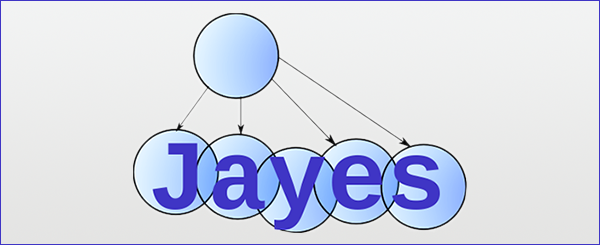
\includegraphics[width=1.0\linewidth]{jayes.png}
\end{figure}

\column{.60\textwidth} % Left column and width

\begin{itemize}
\item Création de réseau bayésien 
\item Calcul d'inférence
\end{itemize}
\end{columns}
\end{frame}
	
	\subsection{Découpage de l'édition de réseaux bayésiens}
	
\begin{frame}
	\frametitle{Découpage de l'édition de réseaux bayésiens}
	
	\begin{enumerate}
	\item étape qualitative : édition du graphe 
	\item étape quantitative : édition des tables de probabilités
	\item étape de simulation : calcul d'inférence
	\end{enumerate}	
	
\end{frame}

%------------------------------------------------
	
	\subsection{Modification de l'interface graphique}
	
\begin{frame}
	\frametitle{Modification de l'interface graphique}
\end{frame}

%------------------------------------------------

\section{Résultats}

%------------------------------------------------

\begin{frame}
\frametitle{Résultats}
\end{frame}

%------------------------------------------------

%----------------------------------------------------------------------------------------

\end{document} 
